\documentclass[11pt]{article}

\usepackage[letterpaper]{geometry}
%\usepackage[letterpaper,left=2.5cm,top=2cm,right=2.5cm,bottom=2cm]{geometry}

\usepackage[utf8]{inputenc}
\usepackage{mathpazo}
\usepackage{amsmath}
\usepackage{amsfonts}
\usepackage{siunitx}
\usepackage{cancel}

\usepackage{graphicx}
\usepackage{float}
\usepackage{empheq}
\usepackage[most]{tcolorbox}

\newtcbox{\mymath}[1][]{%
  nobeforeafter, math upper, tcbox raise base,
  enhanced, colframe=black!30!black,
  colback=yellow!30, boxrule=1pt,
  #1}

% Hyperlinks with decent looking default colors.
\usepackage{hyperref}
\usepackage{xcolor}
\hypersetup{
  colorlinks,
  linkcolor={red!50!black},
  citecolor={blue!50!black},
  urlcolor={blue!80!black}
}

% For those sexy spaced low small caps from classic-thesis!
\usepackage{microtype}
\usepackage{textcase}
\DeclareRobustCommand{\spacedlowsmallcaps}[1]{%
  \textls[80]{\scshape\MakeTextLowercase{#1}}%
}

\usepackage{fancyhdr}
\pagestyle{fancy} 
\fancyhead{}
\rhead{Ali Ramadhan}
\lhead{6.339 Project 1---Finite Difference Methods}
\cfoot{\thepage}

\title{\spacedlowsmallcaps{6.339: Numerical Methods for Partial Differential Equations}\\ \spacedlowsmallcaps{Project one: Finite Difference Methods}}
\author{Ali Ramadhan$^\text{†}$ (\texttt{alir@mit.edu})}
\date{\textit{$^\text{†}$Department of Earth, Atmospheric, and Planetary Sciences}}

\renewcommand\thesection{\Alph{section}}

\begin{document}
\maketitle

In this project, we will utilize finite difference methods to solve the two-dimensional time-dependent Euler equations, a set of quasilinear hyperbolic partial differential equations, for the pressure field of a fluid flowing around a small perturbative bump.

The Euler equations mathematically represent the conservation of mass and momentum for a fluid and can be used to describe the flow of an inviscid fluid, that is a fluid with zero viscosity. Incompressible and compressible formulations both exist, with the latter allowing for sound waves. The governing equations employed in this project follow from the compressible formulation.

Before tackling the questions, I will first introduce the finite difference operators that I use. A second-order finite-difference approximation for the first derivative of an arbitrary real-valued and sufficiently differentiable multivariable function $f = f(x)$ on a grid, as we saw in class, would be 
\begin{equation} \label{eq:firstD}
\frac{df(x_i)}{dx} = \frac{f(x_{i+1}) - f(x_{i-1})}{2\Delta x} + \mathcal{O}(\Delta x)^2
\end{equation}
where $\Delta x$ is the spacing between two successive uniformly distributed grid points, while the second derivative can be approximated as
\begin{equation} \label{eq:secondD}
\frac{d^2 f(x_i)}{dx^2} = \frac{f(x_{i+1}) - 2f(x_i) + f(x_{i-1})}{(\Delta x)^2} + \mathcal{O}(\Delta x)^2
\end{equation}
as we also saw in class, and together they can be used to discretize the governing Euler equations in space. Both finite difference operators \eqref{eq:firstD} and \eqref{eq:secondD} accurately approximate the derivatives up to a truncation error on the order of $(\Delta x)^2$, thus their classification as second-order operators. It will also be useful at certain points to introduce the second-order forward difference operator
\begin{equation} \label{eq:firstDforward}
\frac{df(x_i)}{dx} = \frac{-3f(x_{i}) + 4f(x_{i+1}) - f(x_{i+2})}{2\Delta x} + \mathcal{O}(\Delta x)^2
\end{equation}
along with the second-order backward difference operator
\begin{equation} \label{eq:firstDbackward}
\frac{df(x_i)}{dx} = \frac{3f(x_{i}) - 4f(x_{i-1}) + f(x_{i-2})}{2\Delta x} + \mathcal{O}(\Delta x)^2
\end{equation}
and the second-order mixed derivative operator assuming that $f$ is now a multivariable function $f = f(x,y)$ with sufficiently smooth derivatives,
\begin{equation} \label{eq:mixedD}
\frac{\partial^2 f_{i,j}}{\partial x \partial y} = \frac{f_{i+1,j+1} - f_{i+1,j-1} - f_{i-1,j+1} + f_{i-1,j-1}}{4\Delta x \Delta y} + \mathcal{O}(\Delta x^2, \Delta y^2)
\end{equation}
where we have introduced the shorthand notation $f(x_i,y_j) \equiv f_{i,j}$ for brevity. We will continue to use this notation throughout the report. The last three finite difference operators represented by equations \eqref{eq:firstDforward}, \eqref{eq:firstDbackward}, and \eqref{eq:mixedD} were not derived in class and so I have derived them in the appendix at the end of this report. \\

\begin{tcolorbox}
  \textit{Question 1(a)---Derive the governing boundary condition for $p'$ on boundary. The error in the boundary condition you derived should be the same as that in the linearized Euler equation.}
\end{tcolorbox}

The bottom ($y=0$) and top ($y=H$) boundary conditions read
\begin{equation} \label{eq:yBCfull}
\nabla p \cdot \mathbf{n} = -\rho \left( \frac{\partial^2 F}{\partial t^2} + 2u\frac{\partial^2 F}{\partial t \partial x} + u^2 \frac{\partial^2 F}{\partial^2 x} \right)
\end{equation}
where $F(x,t)$ describes the geometry for the lower and upper walls and $\mathbf{n}$ is the normal vector pointing into the flow field such that $\mathbf{n} = (F_x, -1)$ for the top wall and $\mathbf{n} = (-F_x, 1)$ for the bottom wall.

Expanding the gradient term in \eqref{eq:yBCfull} we obtain 
\begin{equation*}
  \nabla p = \nabla(p_0 + p') = \cancelto{0}{\nabla p_0} + \nabla p' = \nabla p'
\end{equation*}
where $\nabla p_0 = 0$ as $p_0$ represents the unperturbed pressure field which does not vary in time or space for our problem. Now expanding the right hand side of \eqref{eq:yBCfull} gives us
\begin{align*}
  \nabla p' \cdot \mathbf{n}
  &= -(\rho_0 + \rho') \left[ \frac{\partial^2 F}{\partial t^2} + 2(u_0 + u')\frac{\partial^2 F}{\partial t \partial x} + (u_0 + u')^2 \frac{\partial^2 F}{\partial^2 x} \right] \\
  &= -(\rho_0 + \rho') \left( \frac{\partial^2 F}{\partial t^2} + 2u_0 \frac{\partial^2 F}{\partial t \partial x} + \cancelto{0}{2u'\frac{\partial^2 F}{\partial t \partial x}} + u_0^2\frac{\partial^2 F}{\partial^2 x} + \cancelto{0}{2u_0u' \frac{\partial^2 F}{\partial^2 x}} + \cancelto{0}{u'^2 \frac{\partial^2 F}{\partial^2 x}} \right) \\
  &= -\rho_0 \frac{\partial^2 F}{\partial t^2} - 2\rho_0 u_0 \frac{\partial^2 F}{\partial t \partial x} - \rho_0 u_0^2\frac{\partial^2 F}{\partial^2 x} - \cancelto{0}{-\rho' \frac{\partial^2 F}{\partial t^2}} - \cancelto{0}{2\rho' u_0 \frac{\partial^2 F}{\partial t \partial x}} - \cancelto{0}{\rho' u_0^2\frac{\partial^2 F}{\partial^2 x}}
\end{align*}
where each slashed out term vanishes to zero as they represent terms with truncation error $\mathcal{O}(p'^2)$. Let me explain. Since all the perturbed quantities, including $p'$, are the result of the bump perturbation in $F$, if we assume that the effect of small perturbations is linear in $F$, then $p'$ and $F$ are of the same order. The same holds true for the other perturbed quantities: $u'$ and $F$ are of the same order, and so are $\rho'$ and $F$. Thus any term involving the product of a perturbed quantity and a derivation of $F$ would have truncation error $\mathcal{O}(p'^2)$ and can be ignored for the purposes of this project. The boundary condition now reads
\begin{equation*}
    \pm \cancelto{0}{\frac{\partial p'}{\partial x}\frac{\partial F}{\partial x}} \mp \frac{\partial p'}{\partial y} = -\rho_0 \left( \frac{\partial^2 F}{\partial t^2} + 2u_0 \frac{\partial^2 F}{\partial t \partial x} + u_0^2\frac{\partial^2 F}{\partial^2 x} \right)
\end{equation*}
where once again the slashed terms vanish as they are small second-order terms. Thus we are left with a boundary condition that reads 
\begin{equation} \label{eq:yBCwitht}
 \mp \frac{\partial p'}{\partial y} = -\rho_0 \left( \frac{\partial^2 F}{\partial t^2} + 2u_0 \frac{\partial^2 F}{\partial t \partial x} + u_0^2\frac{\partial^2 F}{\partial^2 x} \right)
\end{equation}
where the $+$ branch is taken for the $y=0$ boundary, and the $-$ branch is taken for the $y=H$ boundary. The boundary condition is accurate up to a truncation error of order $p'^2$ as required. \\

\begin{tcolorbox}
  \textit{Question 1(b)---Derive a numerical scheme for the governing equation, using second-order finite-difference in space.}
\end{tcolorbox}
Taking a look at $p' = p'(x,y,t)$ first, which is the perturbed pressure field of the fluid flow, its governing equation can be written as
\begin{equation}
  \frac{\partial p'}{\partial t} + \mathbf{u}_0 \cdot \nabla p' = q'
\end{equation}
where $\mathbf{u}_0 = (u_0, v_0)$ is the unperturbed fluid flow velocity vector and
\begin{equation*}
  q' = \frac{Dp'}{Dt} \equiv \frac{\partial p'}{\partial t} + \mathbf{u}_0 \cdot \nabla p'
\end{equation*}
is the \emph{material derivative} of $p'$. Expanding the dot product and gradient, the governing equation can be written as
\begin{equation} \label{eq:govpp}
\frac{\partial p'}{\partial t} = q' - u_0 \frac{\partial p'}{\partial x} - v_0 \frac{\partial p'}{\partial y}
\end{equation}
where we haved moved the $\mathbf{u}_0 \nabla p'$ term to the right hand side. Now we can discretize the spatial derivatives using \eqref{eq:firstD} to obtain
\begin{empheq}[box=\mymath]{equation} \label{eq:ppDisc}
  \frac{dp'_{i,j}}{dt} = q'_{i,j} - u_0\frac{p'_{i+1,j} - p'_{i-1,j}}{2\Delta x} - v_0 \frac{p'_{i,j+1} - p'_{i,j-1}}{2\Delta y}.
\end{empheq}

The corresponding governing equation for $q'$ is
\begin{equation}
  \frac{\partial q'}{\partial t} + \mathbf{u}_0 \cdot \nabla q' = c_0^2 \nabla^2 p'
\end{equation}
where $c_0^2$ is the unperturbed speed of sound in the fluid. Expanding the dot product and the Laplacian terms, we arrive at
\begin{equation} \label{eq:govqp}
  \frac{\partial q'}{\partial t} = c_0^2 \left( \frac{\partial^2 p'}{\partial x^2} + \frac{\partial^2 p'}{\partial y^2}\right) - u_0 \frac{\partial q'}{\partial x} - v_0 \frac{\partial q'}{\partial y}
\end{equation}
where again we have moved the $\mathbf{u}_0 \cdot \nabla q'$ term to the right hand side and which we can now discretize using \eqref{eq:firstD} and \eqref{eq:secondD} to obtain
\begin{empheq}[box=\mymath]{multline} \label{eq:qpDisc}
  \frac{\partial q'_{i,j}}{\partial t} = c_0^2 \left( \frac{p'_{i+1,j} - 2p'_{i,j} + p'_{i-1,j}}{(\Delta x)^2} + \frac{p'_{i,j+1} - 2p'_{i,j} + p'_{i,j-1}}{(\Delta y^2)} \right) \\
  - u_0\frac{q'_{i+1,j} - q'_{i-1,j}}{2\Delta x} - v_0 \frac{q'_{i,j+1} - q'_{i,j-1}}{2\Delta y}.
\end{empheq}

Equations \eqref{eq:ppDisc} and \eqref{eq:qpDisc} each provide us with a set of $(N+1)(M+1)$ ordinary differential equations (ODEs) that may be integrated numerically to obtain the values of $p'$ and $q'$ at each grid point as a function of time, but we also require appropriate boundary conditions. Let us look at the boundary conditions for $p'$ first. The left boundary condition reads $p = p_0$ at $x = 0$ but $p = p_0 + p'$ by definition so we must have that $p' = 0$ at $x = 0$ or
\begin{empheq}[box=\mymath]{equation} \label{eq:sameBC1}
  p'_{0,j} = 0 \quad \mathrm{for \; all} \; j
\end{empheq}
The right boundary condition reads $\displaystyle \frac{dp'}{dx'} = 0$ which we can discretize using \eqref{eq:firstD} to get
\begin{equation}
  \frac{p'_{N+1,j} - p'_{N,j}}{2\Delta x} = 0
\end{equation}
or rather, that the boundary grid points must equal the ones to their left,
\begin{empheq}[box=\mymath]{equation} \label{eq:sameBC2}
   p'_{N+1,j} = p'_{N,j} \quad \mathrm{for \; all} \; j
\end{empheq}

The bottom ($y=0$) boundary condition is described by the $+$ branch of \eqref{eq:yBCwitht}, however $F(x,t) = F(x)$, a function of space only, along the $y=0$ boundary and thus the condition simplifies to
\begin{equation}
  \frac{\partial p'}{\partial y} = -\rho_0 u_0^2 \frac{\partial^2 F}{\partial x^2}
\end{equation}
which can be discretized as
\begin{equation}
\frac{p'_{i,2} - p'_{i,1}}{2\Delta y} = -\rho_0 u_0^2 \frac{F_{i+1} - 2F_i + F_{i-1}}{(\Delta x)^2}
\end{equation}
or solved for the boundary values $p'_{i,1}$ to get
\begin{empheq}[box=\mymath]{equation}
p'_{i,1} = p'_{i,2} + 2\rho_0 u_0^2 \frac{F_{i+1} - 2F_i + F_{i-1}}{(\Delta x)^2}\Delta y  \quad \mathrm{for \; all} \; i
\end{empheq}
Note that $F(x)$ for our problem is only non-zero for $L/4 < x_i < L/2$, and thus for $x < L/4$ and $x > L/2$, the condition will simplify to $p'_{i,1} = p'_{i,2}$. The top ($y=H$) boundary condition is described by the $-$ branch of \eqref{eq:yBCwitht} but $F(x,t) = H$, a constant value, at $y=H$ and thus the condition simplifies greatly to
\begin{equation}
  \frac{p'_{i,M+1} - p'_{i,M}}{2\Delta y} = 0
\end{equation}
or, since we are interested in the value at the boundary,
\begin{empheq}[box=\mymath]{equation}
p'_{i,M+1} = p'_{i,M} \quad \mathrm{for \; all} \; i
\end{empheq}

Now taking a look at the boundary conditions for $q'$, the condition on the left wall reads $q' = 0$ at $x = 0$ which may be easily discretized as
\begin{empheq}[box=\mymath]{equation} \label{eq:sameBC3}
  q'_{0,j} = 0 \quad \mathrm{for \; all} \; j
\end{empheq}
while the condition for $q'$ on the right wall ($x=L$) reads $\displaystyle \frac{dq'}{dx'} = 0$ which can be easily discretized just like its $p'$ conterpart to obtain
\begin{empheq}[box=\mymath]{equation} \label{eq:sameBC4}
q'_{N+1,j} = q'_{N,j} \quad \mathrm{for \; all} \; j
\end{empheq} \\

\begin{tcolorbox}
  \textit{Question 2(a)---On a bump described by function:}
  \begin{equation*}
    F(x) = 0.01 \left\{ 1 - \cos \left[ \frac{8\pi}{L} \left( x - \frac{L}{4} \right) \right] \right\}^2
  \end{equation*}
  \textit{Plot the contour for $p'$ at time $t=2$ in your report (no figure
  generation in submitted code). Include the color-bar in the figure.}
\end{tcolorbox}
Taking the yellow boxed equations representing the time evolution of each grid point $p'_{i,j}$ and $q'_{i,j}$ along with the boundary conditions determined by the given form for $F(x)$ and assuming that $v_0=0$ as the unperturbed fluid flows only in the horizontal direction, we can use the \texttt{ode45} function in MATLAB to integrate the discretized equations and obtain the desired pressure field at $t=2$, shown in figure \ref{fig:pp_q2_contourf}. We see a high pressure region to the left of the bump followed by a high pressure region to the right of the bump. The zero-pressure line seems to originate at the peak of the bump perturbation ($x = 3L/8 = 2.25$). \\

\begin{figure}
  \centering
  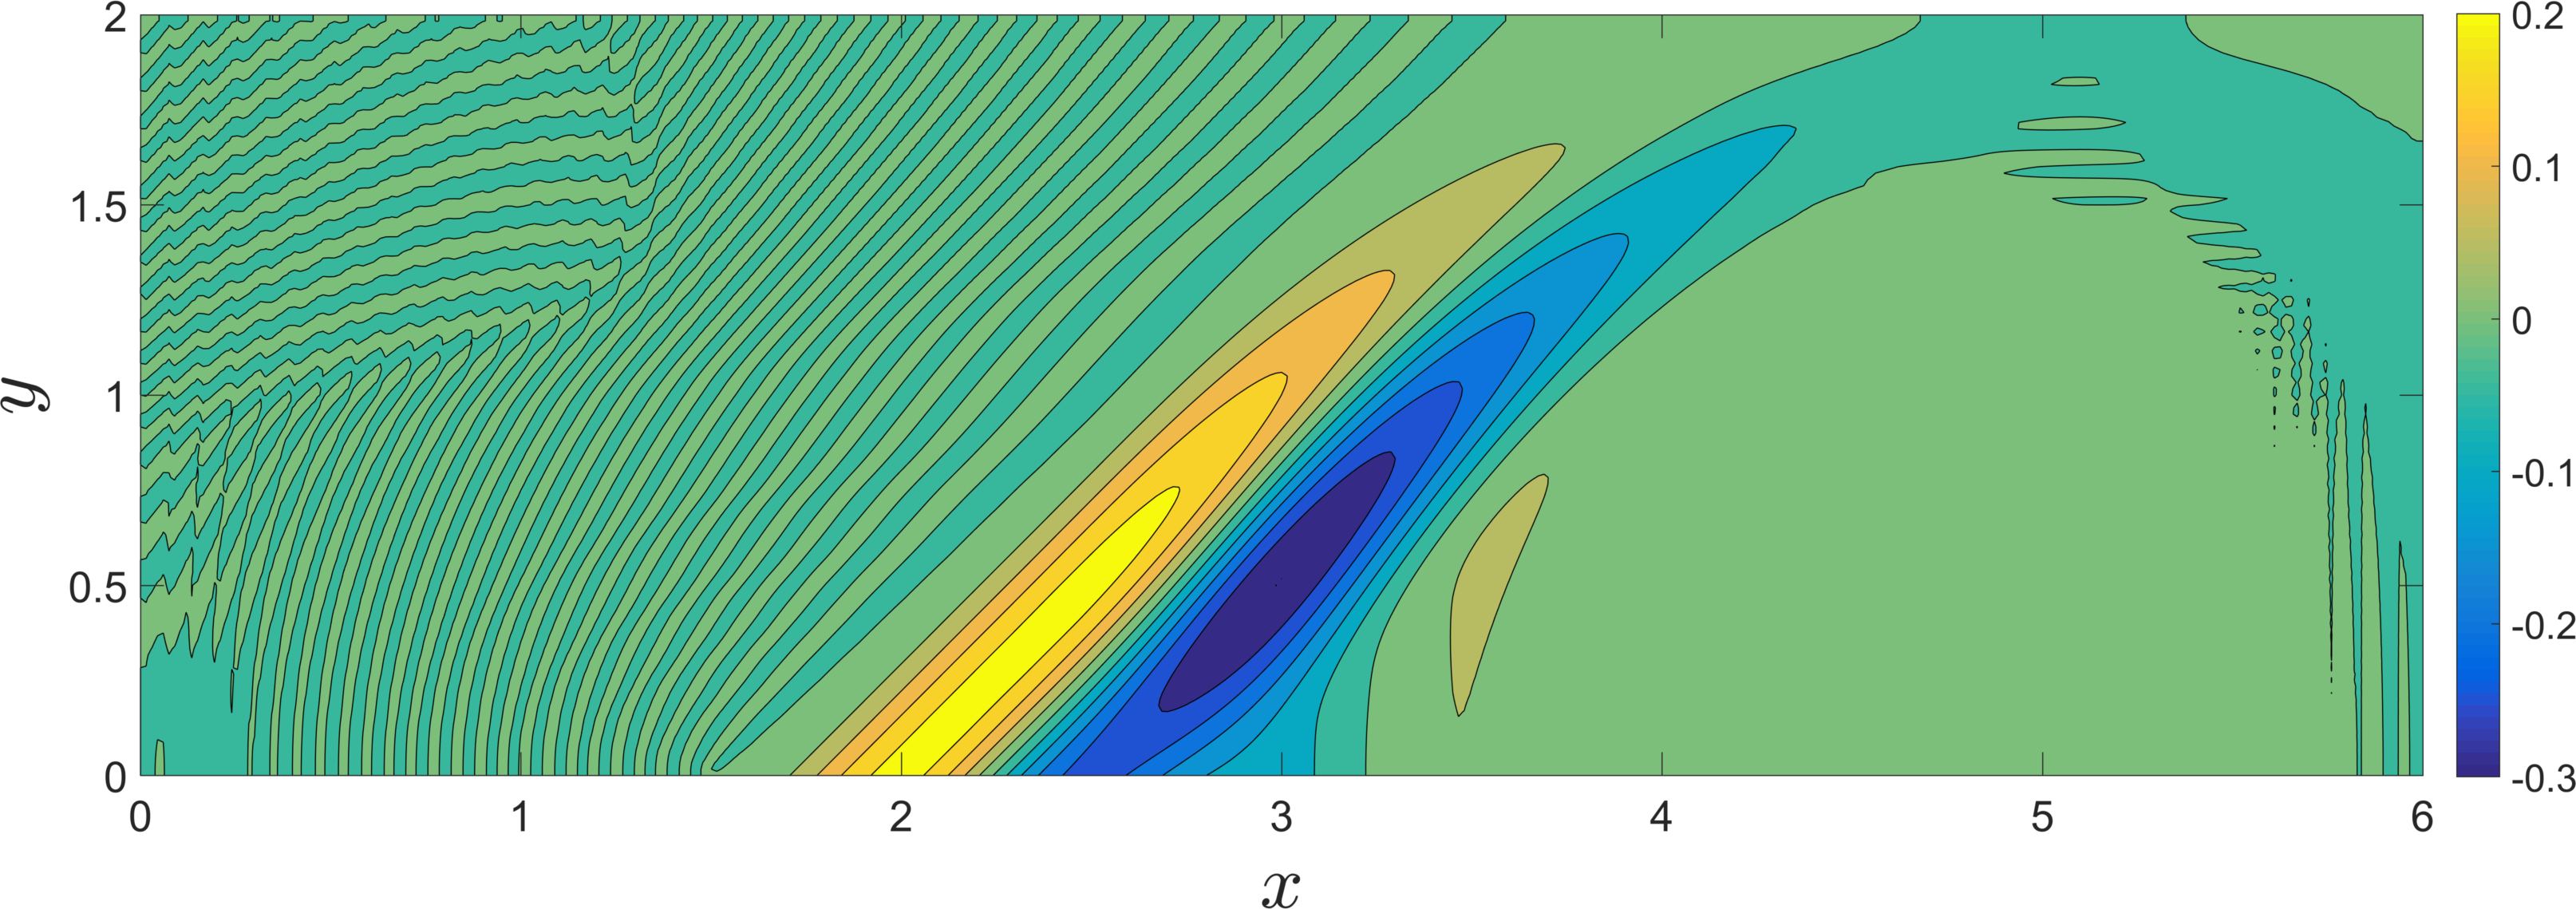
\includegraphics[width=\textwidth]{pp_q2_contourf.png}
  \caption{The perturbed pressure field $p'(x,y,t)$ at $t=2$. A mesh size of $N=400$ and $M=120$ was used.}
  \label{fig:pp_q2_contourf}
\end{figure}

\begin{tcolorbox}
  \textit{Question 3(a)---Estimate what the twist angle $\theta$ should be, so that the mesh aligns with the features of the solution.}
\end{tcolorbox}
We can manually measure the angle from figure 1. Choosing a vector $\mathbf{x}_1 = (1.74, 0)$ from the origin to the bottom left corner of the high pressure region to the left of the bump, and another vector $\mathbf{x}_2 = (1.14, 1.133)$ from $\mathbf{x}_1$ to along the high pressure region's straight left boundary, we can calculate the angle between the two vector using
\begin{equation*}
  \theta = \arccos \frac{\mathbf{x}_1 \cdot \mathbf{x}_2}{\left\lVert\mathbf{x}_1\right\rVert \left\lVert\mathbf{x}_2\right\rVert} \approx \frac{\pi}{4}
\end{equation*}
which results in an angle very close to $45^\circ$. Thus it makes sense to choose $\theta = \pi/4$ for the oblique mesh. \\

\begin{tcolorbox}
  \textit{Question 3(b)---Derive the governing equation on this new mesh.}
\end{tcolorbox}
To do so we will make a coordinate transformation from Cartesian coordinates $(x,y)$ to the oblique coordinate system, which we will denote by $(\tilde{x}, \tilde{y})$. The transformation is given by
\begin{subequations}
\begin{align}
  \tilde{x} &= x - y\tan\theta \\
  \tilde{y} &= y\sec\theta
\end{align}
\end{subequations}
which will transform the differential operators according the chain rule,
\begin{align*}
  \frac{\partial f}{\partial x} &= \frac{\partial f}{\partial \tilde{x}} \frac{\partial \tilde{x}}{\partial x}
  + \frac{\partial f}{\partial \tilde{y}} \frac{\partial \tilde{y}}{\partial x} = \frac{\partial f}{\partial \tilde{x}} \\
  \frac{\partial f}{\partial y} &= \frac{\partial f}{\partial \tilde{x}} \frac{\partial \tilde{x}}{\partial y}
  + \frac{\partial f}{\partial \tilde{y}} \frac{\partial \tilde{y}}{\partial y} = -\tan\theta\frac{\partial f}{\partial \tilde{x}} + \sec\theta \frac{\partial f}{\partial \tilde{y}}
\end{align*}
so that they can be substituted by differential operators with respect to the oblique coordinate system
\begin{subequations}
\begin{align}
  \frac{\partial}{\partial x} &\rightarrow \frac{\partial}{\partial \tilde{x}} \label{eq:NewDOx} \\
  \frac{\partial}{\partial y} &\rightarrow -\tan\theta\frac{\partial}{\partial \tilde{x}} + \sec\theta\frac{\partial}{\partial \tilde{y}} \label{eq:NewDOy}
\end{align}
\end{subequations}

Substituting our new differential operators \eqref{eq:NewDOx} and \eqref{eq:NewDOy} into the governing equation for $p'$ \eqref{eq:govpp} we get
\begin{equation} \label{eq:govppTilde}
\frac{\partial p'}{\partial t} = q' - u_0 \frac{\partial p'}{\partial \tilde{x}} - v_0 \left( -\tan\theta \frac{\partial p'}{\partial \tilde{x}} + \sec\theta  \frac{\partial p'}{\partial \tilde{y}} \right)
\end{equation}
and doing the same for the governing equation for $q'$ \eqref{eq:govqp} we get
\begin{multline} \label{eq:govqpTilde}
\frac{\partial q'}{\partial t} =
  c_0^2 \left( \sec^2\theta \frac{\partial^2 p'}{\partial \tilde{x}^2} + \sec^2\theta \frac{\partial^2 p'}{\partial \tilde{y}^2} - 2\sec\theta\tan\theta \frac{\partial^2 p'}{\partial\tilde{x} \partial\tilde{y}} \right) \\
  - u_0 \frac{\partial q'}{\partial \tilde{x}}
  - v_0 \left( -\tan\theta \frac{\partial q'}{\partial \tilde{x}} + \sec\theta \frac{\partial p'}{\partial \tilde{y}} \right)
\end{multline}

The boundary condition at the bottom wall \eqref{eq:yBCwitht} at $\tilde{y}=0$ now becomes more complicated involving multiple derivatives,
\begin{equation} \label{eq:y0BCoblique}
\tan\theta \frac{\partial p'}{\partial \tilde{x}} - \sec\theta \frac{\partial p'}{\partial \tilde{y}} = -\rho_0 u_0^2 \frac{\partial^2F}{\partial \tilde{x}^2}, \quad \frac{L}{4} < \tilde{x} < \frac{L}{2}
\end{equation}
otherwise the right hand side is zero for $\tilde{x} < L/2$ and $\tilde{x} > L/2$. On the other hand, the boundary condition at the top wall \eqref{eq:yBCwitht} at $y=H$, or $\tilde{y}=H\sec\theta$ is slightly simpler,
\begin{equation} \label{eq:yHoblique}
  \tan\theta \frac{\partial p'}{\partial \tilde{x}} - \sec\theta \frac{\partial p'}{\partial \tilde{y}} = 0
\end{equation}

\begin{tcolorbox}
  \textit{Question 3(c)---Derive a numerical scheme for the governing equation, using second-order finite-difference in space.}
\end{tcolorbox}
We will again take $v_0 = 0$, which will simplify the governing equations. Using the central difference finite-difference operator \eqref{eq:firstD} for the first derivative we can discretize the governing equation for $p'$ in the oblique coordinate system \eqref{eq:govppTilde} as
\begin{empheq}[box=\mymath]{equation} \label{eq:ppDiscTilde}
\frac{dp'_{i,j}}{dt} = q'_{i,j} - u_0\frac{p'_{i+1,j} - p'_{i-1,j}}{2\Delta \tilde{x}}
\end{empheq}
and results in exactly the same discretization used previously [see equation \eqref{eq:ppDisc}]. Utilizing the finite-difference operator for the second derivative \eqref{eq:secondD} and the finite-difference operator for the mixed second derivative \eqref{eq:mixedD} we can also discretize the governing equation for $q'$ in the oblique coordinate system as
\begin{empheq}[box=\mymath]{multline} \label{eq:qpDiscTilde}
\frac{\partial q'_{i,j}}{\partial t} =
  c_0^2 \left(
    \sec^2\theta \frac{p'_{i+1,j} - 2p'_{i,j} + p'_{i-1,j}}{(\Delta \tilde{x})^2}
    + \sec^2\theta \frac{p'_{i,j+1} - 2p'_{i,j} + p'_{i,j-1}}{(\Delta \tilde{y}^2)} \right. \\ \left.
    - 2\sec\theta\tan\theta \frac{p'_{i+1,j+1} - p'_{i+1,j-1} - p'_{i-1,j+1} + p'_{i-1,j-1}}{4\Delta\tilde{x}\Delta\tilde{y}} \right)
- u_0\frac{q'_{i+1,j} - q'_{i-1,j}}{2\Delta\tilde{x}}.
\end{empheq}

The boundary conditions require some more work to discretize. The presence of multiple derivatives leads to boundary values that depend on other boundary values, turning the problem of calculating the boundary values from just arithmetic to solving a system of linear equations. Using a second-order backward difference operator, the $\tilde{y}=H$ boundary condition \eqref{eq:yHoblique} can be written as a system of $N+1$ linear equations for the value of $p'$, or more specifically, for the $N+1$ unknown values $p'_{i,M+1}$ along the $\tilde{y}=H$ boundary,
\begin{empheq}[box=\mymath]{equation}
  \frac{\tan\theta}{2\Delta\tilde{x}} p'_{i-1,M+1}
  + \frac{3\sec\theta}{2\Delta\tilde{y}} p'_{i,M+1}
  - \frac{\tan\theta}{2\Delta\tilde{x}} p'_{i+1,M+1}
  = \sec\theta \frac{4p'_{i,M} - p'_{i,M-1}}{2\Delta\tilde{y}}
\end{empheq}
A similar process for the $\tilde{y}=0$ boundary condition, except for the use of a second-order forward difference operator, produces another system of linear equations for the $N+1$ unknown values $p'_{i,1}$ along the $\tilde{y}=0$ boundary,
\begin{empheq}[box=\mymath]{equation}
  \frac{\tan\theta}{2\Delta\tilde{x}} p'_{i-1,1}
- \frac{3\sec\theta}{2\Delta\tilde{y}} p'_{i,1}
- \frac{\tan\theta}{2\Delta\tilde{x}} p'_{i+1,1}
= - \sec\theta \frac{4p'_{i,2} - p'_{i,3}}{2\Delta\tilde{y}}
- \rho_0 u_0^2 \frac{F_{i+1} - 2F_i + F_{i-1}}{(\Delta\tilde{x})^2}
\end{empheq}
both of which may be cast as a matrix equation of the form $A\mathbf{x} = \mathbf{b}$ and easily solved in MATLAB due to their relatively small size. The other four boundary conditions for $p'$ and $q'$ on the left and right walls, represented by equations \eqref{eq:sameBC1}, \eqref{eq:sameBC2}, \eqref{eq:sameBC3}, and \eqref{eq:sameBC4}, remain the same as $\tilde{x}=0$ $\tilde{x}=L$ correspond to $x=0$ and $x=L$ respectively so they can be reused. \\

\begin{tcolorbox}
  \textit{Question 4---Same as question 2.}
\end{tcolorbox}
Again taking the yellow boxed equations from question (3b) representing the time evolution of each grid point $p'_{i,j}$ and $q'_{i,j}$ along with the boundary conditions determined by the given form for $F(x)$ from question 2, we can use the \texttt{ode45} function in MATLAB to integrate the discretized equations and obtain the desired pressure field at $t=2$, shown in figure \ref{fig:pp_q4_contourf}. We again see a high pressure region to the left of the bump followed by a high pressure region to the right of the bump, however, the pressure regions are now straight as they align with the oblique mesh by design.

\begin{figure}[h!]
  \centering
  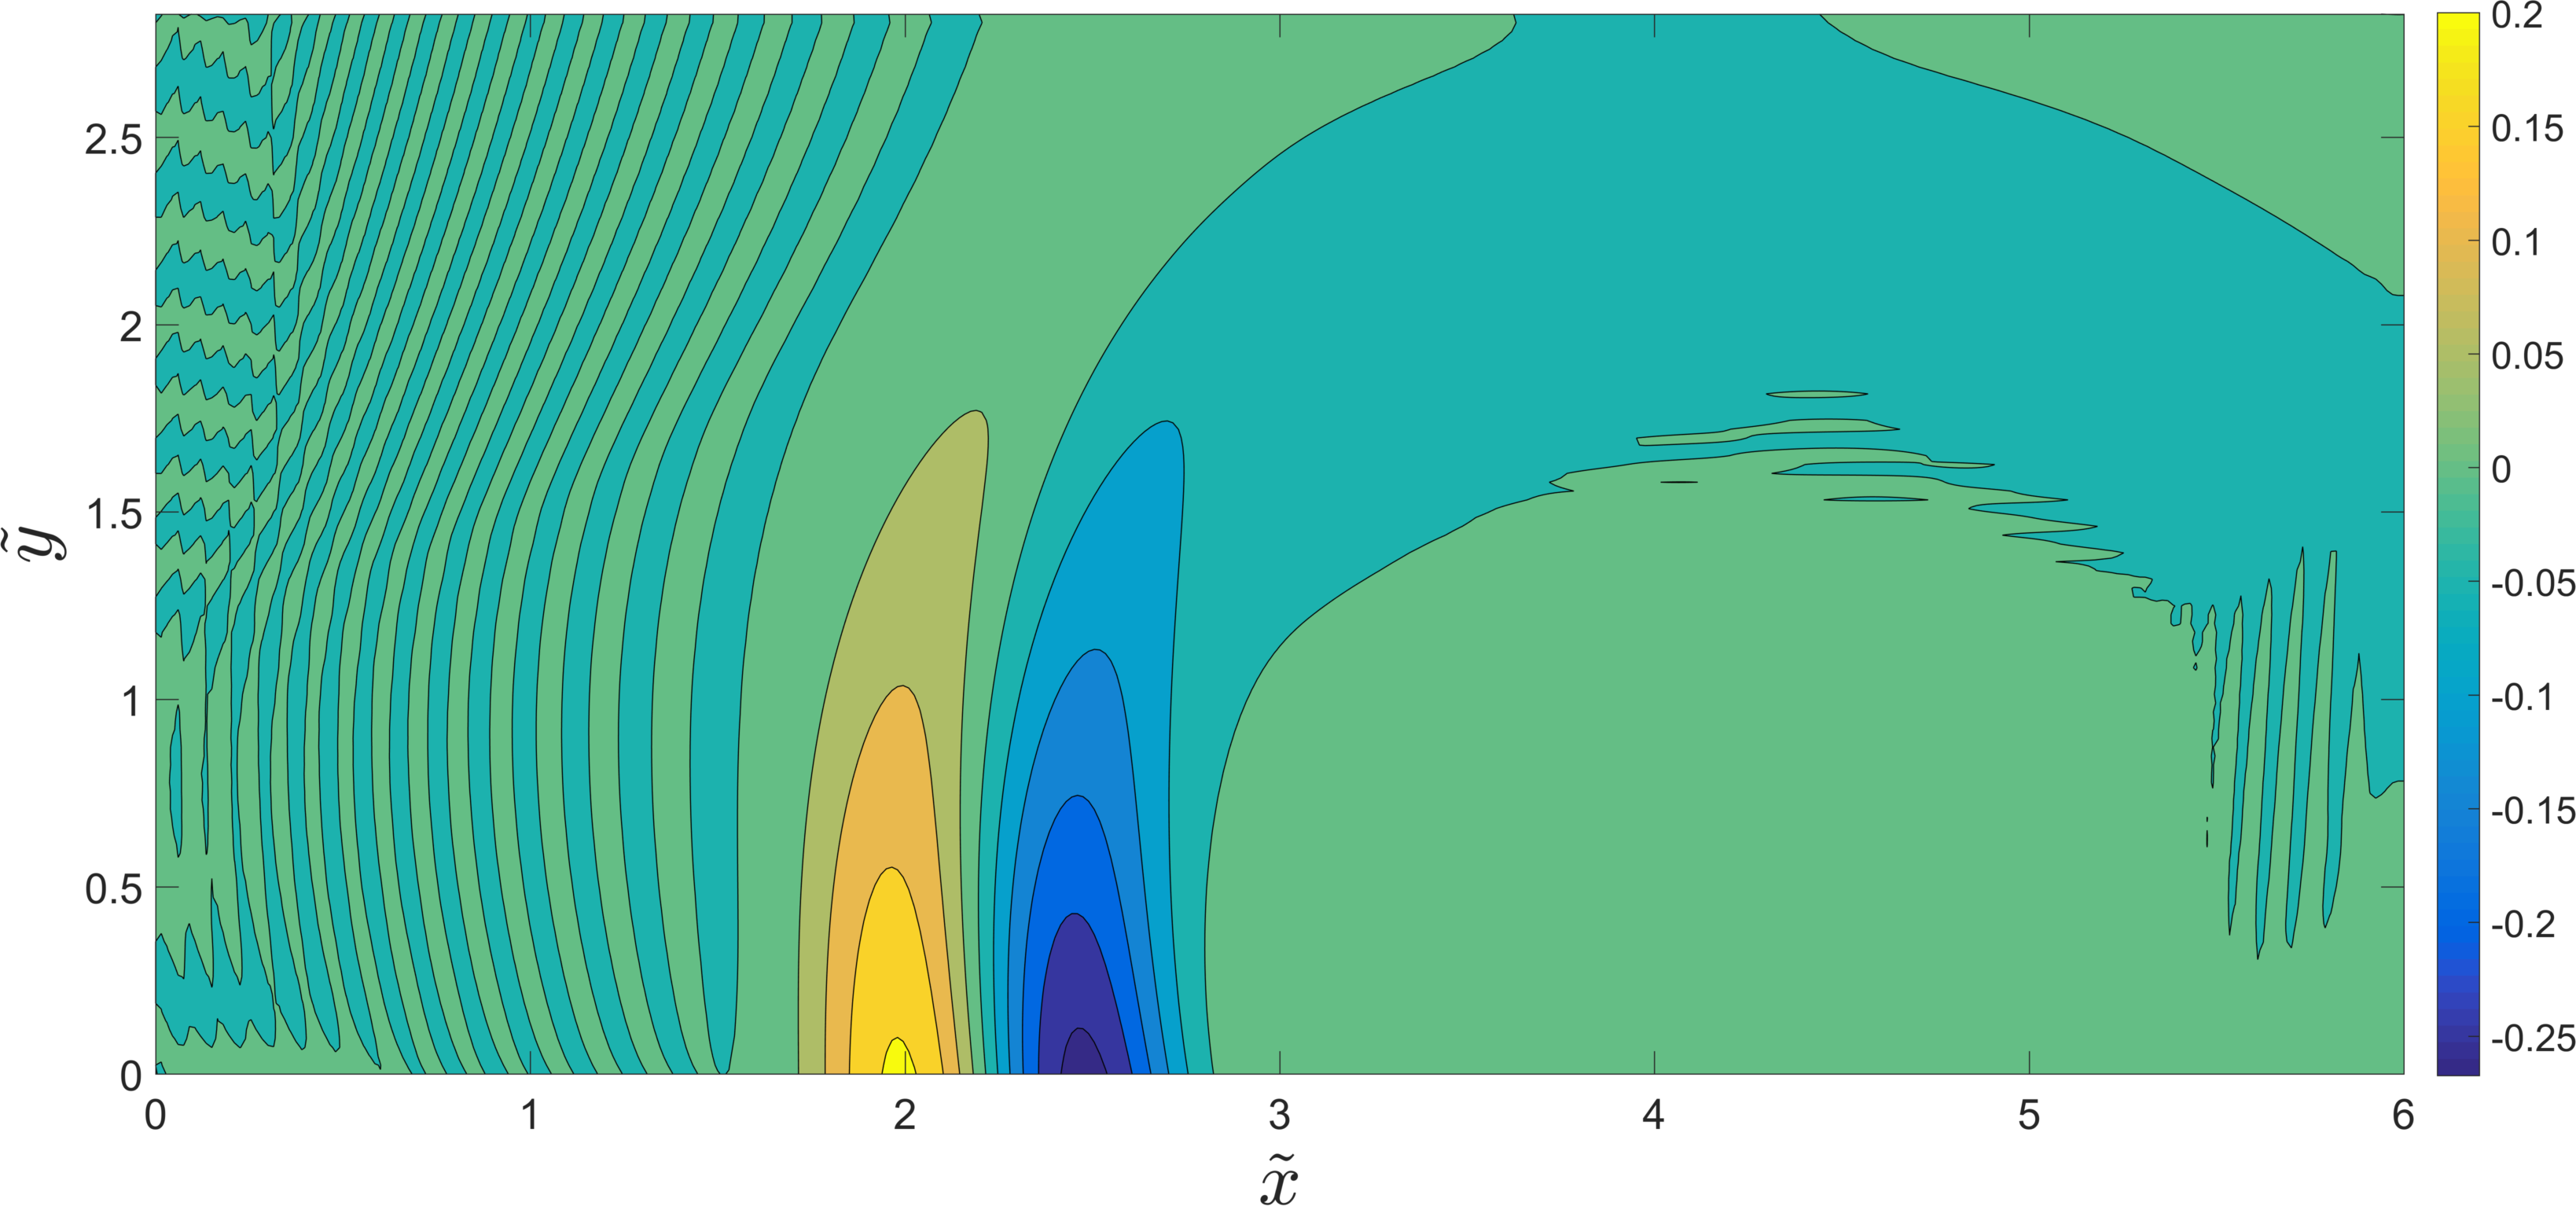
\includegraphics[width=\textwidth]{pp_q4_contourf.png}
  \caption{The perturbed pressure field $p'(\tilde{x},\tilde{y},t)$ at $t=2$. A mesh size of $N=400$ and $M=120$ was used. Note that the vertical domain is now $0 \le \tilde{y} \le H\sec\theta$ so that the top boundary corresponds to $y=H$.}
  \label{fig:pp_q4_contourf}
\end{figure}

\section*{Appendix: derivation of finite difference operators}
Let us first derive the second-order forward and backward finite difference operators for the first derivative which we gave in equations \eqref{eq:firstDforward} and \eqref{eq:firstDbackward}. We will take the same approach we took in class and attempt to find the value of the constants $a$, $b$, and $c$ that minimize
\begin{displaymath}
  af_i + bf_{i\pm 1} + cf_{i\pm 2} - \frac{df(x_i)}{dx}
\end{displaymath}
where the $+$ branch corresponds to the forward operator and the $-$ branch to the backward operator. Expanding $f_{i\pm 1}$ and $f_{i\pm 2}$ as Taylor series about the point $x_i$ we obtain
\begin{multline*}
af_i
+ b\left( f_i \pm \Delta x \frac{df_i}{dx} + \frac{(\Delta x)^2}{2} \frac{d^2f_i}{dx^2} + \mathcal{O}(\Delta x)^3 \right) \\
+ c\left( f_i \pm 2\Delta x \frac{df_i}{dx} + \frac{(2\Delta x)^2}{2} \frac{d^2f_i}{dx^2} + \mathcal{O}(\Delta x)^3 \right) - \frac{df(x_i)}{dx} \\
= (a+b+c)f_i + \left( a \pm b \pm 2c - \frac{1}{\Delta x} \right) \Delta x \frac{df_i}{dx} + \left( \frac{b}{2} + 2c \right) (\Delta x)^2 \frac{d^2f_i}{dx^2} + \mathcal{O}(\Delta x)^3
\end{multline*}
which is minimized when $a+b+c=0$, $a \pm b \pm 2c = 1/\Delta x$, and $b/2 + 2c = 0$. Solving the $+$ branch gives us the forward operator with $a=-3/2\Delta x$, $b=4/2\Delta x$, and $c=-1/2\Delta x$,
\begin{equation}
\frac{df_i}{dx} = \frac{-3f_i + 4f_{i+1} - f_{i+2}}{2\Delta x} + \mathcal{O}(\Delta x)^2
\end{equation}
while solving the $-$ branch gives us the backward operator with $a=3/2\Delta x$, $b=-4/2\Delta x$, and $c=1/2\Delta x$
\begin{equation}
\frac{df_i}{dx} = \frac{3f_{i} - 4f_{i-1} + f_{i-2}}{2\Delta x} + \mathcal{O}(\Delta x)^2
\end{equation}

Repeating this process for the mixed derivative but using a 4-point stencil we wish to minimize
\begin{displaymath}
  af_{i+1,j+1} + bf_{i+1,j-1} + cf_{i-1,j+1} + d_{i-1,j-1} - \frac{f_{i,j}}{\partial x \partial y}
\end{displaymath}
and after expanding each term as a Taylor series about the point $(x_i, y_j)$ we obtain
\begin{multline*}
a \left(
  f_{i,j}
  + \Delta x \frac{\partial f}{\Delta x}
  + \Delta y \frac{\partial f}{\Delta y}
  + \frac{(\Delta x)^2}{2} \frac{\partial^2 f}{\Delta x^2}
  + \frac{(\Delta y)^2}{2} \frac{\partial^2 f}{\Delta y^2}
  + \Delta x \Delta y \frac{\partial^2 f}{\partial x \partial y}
  \right) \\
+ b \left(
f_{i,j}
+ \Delta x \frac{\partial f}{\Delta x}
- \Delta y \frac{\partial f}{\Delta y}
+ \frac{(\Delta x)^2}{2} \frac{\partial^2 f}{\Delta x^2}
+ \frac{(\Delta y)^2}{2} \frac{\partial^2 f}{\Delta y^2}
- \Delta x \Delta y \frac{\partial^2 f}{\partial x \partial y}
\right) \\
+ c \left(
f_{i,j}
- \Delta x \frac{\partial f}{\Delta x}
+ \Delta y \frac{\partial f}{\Delta y}
+ \frac{(\Delta x)^2}{2} \frac{\partial^2 f}{\Delta x^2}
+ \frac{(\Delta y)^2}{2} \frac{\partial^2 f}{\Delta y^2}
- \Delta x \Delta y \frac{\partial^2 f}{\partial x \partial y}
\right) \\
+ d \left(
f_{i,j}
- \Delta x \frac{\partial f}{\Delta x}
- \Delta y \frac{\partial f}{\Delta y}
+ \frac{(\Delta x)^2}{2} \frac{\partial^2 f}{\Delta x^2}
+ \frac{(\Delta y)^2}{2} \frac{\partial^2 f}{\Delta y^2}
+ \Delta x \Delta y \frac{\partial^2 f}{\partial x \partial y}
\right) \\
+ \mathcal{O}(\Delta x^3, \Delta y^3) - \frac{\partial^2 f}{\partial x \partial y}
\end{multline*}
where $f \equiv f_{i,j}$ in the derivatives for brevity, which can be factored as
\begin{multline*}
(a + b + c + d)f_{i,j}
  + (a + b - c - d) \Delta x \frac{\partial f}{\Delta x}
  + (a - b + c - d) \Delta y \frac{\partial f}{\Delta y} \\
  + (a + b + c + d) \frac{(\Delta x)^2}{2} \frac{\partial^2 f}{\Delta x^2}
  + (a + b + c + d) \frac{(\Delta y)^2}{2} \frac{\partial^2 f}{\Delta y^2} \\
  + \left(a - b - c + d - \frac{1}{\Delta x \Delta y} \right) \Delta x \Delta y \frac{\partial^2 f}{\partial x \partial y} + \mathcal{O}(\Delta x^3, \Delta y^3)
\end{multline*}
and is minimized when $a+b+c+d=0$, $a+b-c-d=0$, $a-b+c-d=0$, and $a-b-c+d=1/\Delta x \Delta y$. Solving this system gives us $a = d = 1/4\Delta x \Delta y$ and $b = c = -1/4\Delta x \Delta y$ and the second-order operator for the mixed second derivative,
\begin{equation}
\frac{\partial^2 f_{i,j}}{\partial x \partial y} = \frac{f_{i+1,j+1} - f_{i+1,j-1} - f_{i-1,j+1} + f_{i-1,j-1}}{4\Delta x \Delta y} + \mathcal{O}(\Delta x^2, \Delta y^2)
\end{equation}

\end{document}